%%%%%%%%%%%%%%%%%%%%%%%%%%%%%%%%%%%%%%%%%
% Beamer Presentation
% LaTeX Template
% Version 1.0 (10/11/12)
%
% This template has been downloaded from:
% http://www.LaTeXTemplates.com
%
% License:
% CC BY-NC-SA 3.0 (http://creativecommons.org/licenses/by-nc-sa/3.0/)
%
%%%%%%%%%%%%%%%%%%%%%%%%%%%%%%%%%%%%%%%%%

%----------------------------------------------------------------------------------------
%	PACKAGES AND THEMES
%----------------------------------------------------------------------------------------

\documentclass{beamer}

\mode<presentation> {

% The Beamer class comes with a number of default slide themes
% which change the colors and layouts of slides. Below this is a list
% of all the themes, uncomment each in turn to see what they look like.

%\usetheme{default}
%\usetheme{AnnArbor}
%\usetheme{Antibes}
%\usetheme{Bergen}
\usetheme{Berkeley}
%\usetheme{Berlin}
%\usetheme{Boadilla}
%\usetheme{CambridgeUS}
%\usetheme{Copenhagen}
%\usetheme{Darmstadt}
%\usetheme{Dresden}
%\usetheme{Frankfurt}
%\usetheme{Goettingen}
%\usetheme{Hannover}
%\usetheme{Ilmenau}
%\usetheme{JuanLesPins}
%\usetheme{Luebeck}
%\usetheme{Madrid}
%\usetheme{Malmoe}
%\usetheme{Marburg}
%\usetheme{Montpellier}
%\usetheme{PaloAlto}
%\usetheme{Pittsburgh}
%\usetheme{Rochester}
%\usetheme{Singapore}
%\usetheme{Szeged}
%\usetheme{Warsaw}

% As well as themes, the Beamer class has a number of color themes
% for any slide theme. Uncomment each of these in turn to see how it
% changes the colors of your current slide theme.

%\usecolortheme{albatross}
%\usecolortheme{beaver}
%\usecolortheme{beetle}
%\usecolortheme{crane}
%\usecolortheme{dolphin}
%\usecolortheme{dove}
%\usecolortheme{fly}
%\usecolortheme{lily}
%\usecolortheme{orchid}
%\usecolortheme{rose}
%\usecolortheme{seagull}
%\usecolortheme{seahorse}
%\usecolortheme{whale}
%\usecolortheme{wolverine}

%\setbeamertemplate{footline} % To remove the footer line in all slides uncomment this line
%\setbeamertemplate{footline}[page number] % To replace the footer line in all slides with a simple slide count uncomment this line

%\setbeamertemplate{navigation symbols}{} % To remove the navigation symbols from the bottom of all slides uncomment this line
}

\usepackage{graphicx} % Allows including images
\usepackage{booktabs} % Allows the use of \toprule, \midrule and \bottomrule in tables
\usepackage{caption}
\usepackage{subcaption}

%----------------------------------------------------------------------------------------
%	TITLE PAGE
%----------------------------------------------------------------------------------------

\title[Short title]{Home Credit Default Risk Prediction} % The short title appears at the bottom of every slide, the full title is only on the title page

\author{Huiwen Wu} % Your name
\institute[UCI] % Your institution as it will appear on the bottom of every slide, may be shorthand to save space
{
University of California, Irvine \\ % Your institution for the title page
\medskip
\textit{huiwenw@uci.edu} % Your email address
}
\date{\today} % Date, can be changed to a custom date

\begin{document}

\begin{frame}
\titlepage % Print the title page as the first slide
\end{frame}

\begin{frame}
\frametitle{Overview} % Table of contents slide, comment this block out to remove it
\tableofcontents % Throughout your presentation, if you choose to use \section{} and \subsection{} commands, these will automatically be printed on this slide as an overview of your presentation
\end{frame}

%----------------------------------------------------------------------------------------
%	PRESENTATION SLIDES
%----------------------------------------------------------------------------------------

%------------------------------------------------
\section{First Section} % Sections can be created in order to organize your presentation into discrete blocks, all sections and subsections are automatically printed in the table of contents as an overview of the talk
%------------------------------------------------

\subsection{Subsection Example} % A subsection can be created just before a set of slides with a common theme to further break down your presentation into chunks

\begin{frame}
\frametitle{Background}
Many people struggle to get loans due to insufficient or non-existent credit histories. And, unfortunately, this population is often taken advantage of by untrustyworthy lenders. 

Home Credit strives to broaden financial inclusion for the unbanked population by providing a positive and safe borrowing experience. In order to make sure this underserved population has a positive loan experience. A variety of alternative data -- including telco and transactional information -- are used to predict clients' repayment abilities. 
\end{frame}

%------------------------------------------------

\begin{frame}
\frametitle{Mathmetical Problems}
\begin{itemize}
\item Input: Data of applications, bureau, credit card, installments payments, POS CASH and previous applications.
\item Output: Probability of clients' ability of loan repayment, a value from 0 to 1. 
\item Probelm: Regression or Classification? 
\end{itemize}


\end{frame}

%-----------------------------------------------
\begin{frame}
\frametitle{Data}
\begin{figure}
  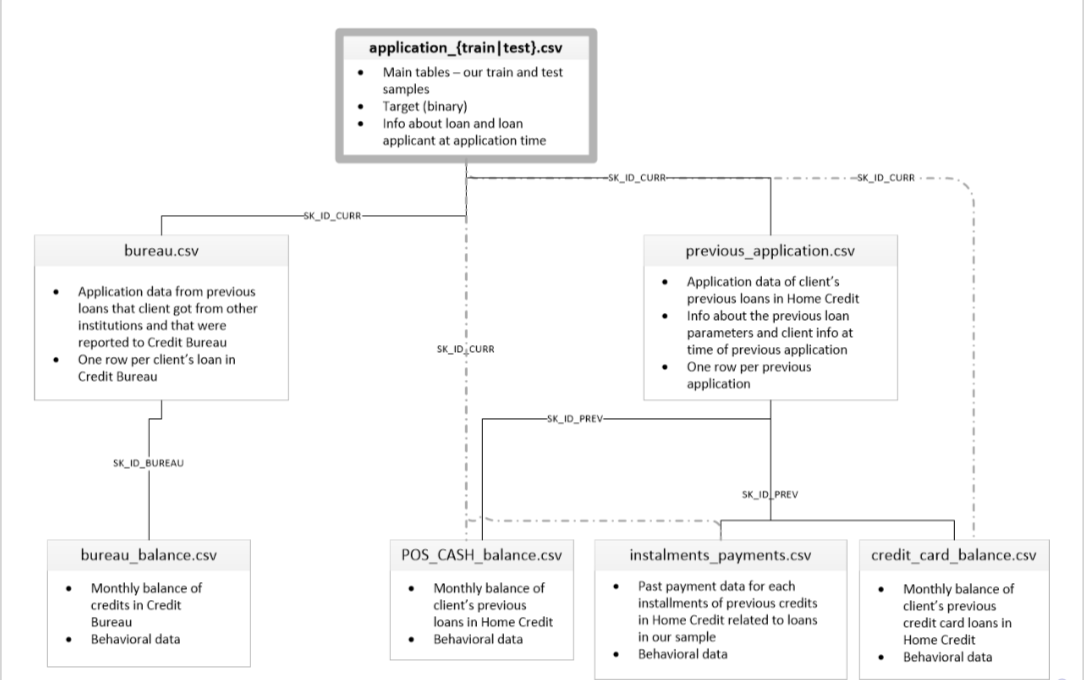
\includegraphics[width=\linewidth]{pic/Home_Credit_data.png}
  \caption{Home Credit Data}
  \label{fig:data}
\end{figure}
\end{frame}

\begin{frame}{Data Characteristics}
\begin{itemize}
\item Massive data and a lot of features $799$. 
\item Redundant information. 
\item A lot of sparse features. 
\item High correlation between some features -- number of children, house type, ages. 
\end{itemize}
\end{frame}
%------------------------------------------------
\section{Models}

\begin{frame}{Logistic Regression}
Logistic Regression uses logistic function to estimate probability. 
$$
c(\theta) = 
\begin{cases}
- \log(h_{\theta}(x)) \quad \quad y = 1 \\
- \log (1 - h_{\theta}(x)) \quad \quad y = 0. 
\end{cases}
$$

\begin{figure}
  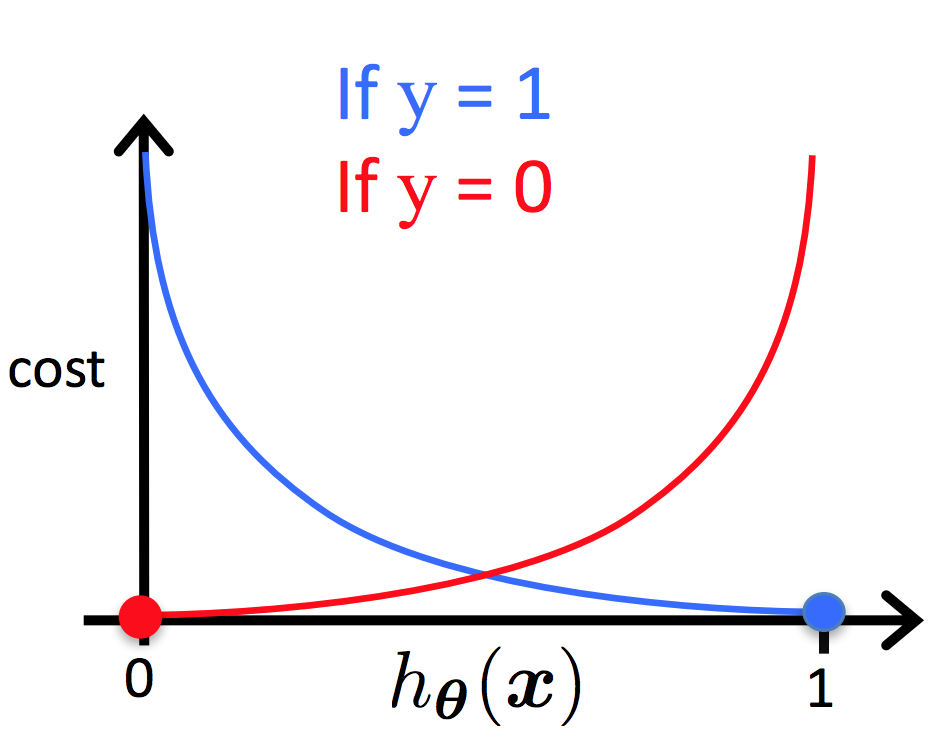
\includegraphics[width=0.6\linewidth]{pic/cost_lr.png}
  \caption{LR Cost Functions}
  \label{fig:cost_lr}
\end{figure}

\end{frame}

\begin{frame}{Decision Tree}
A decision tree is a decision support tool that uses a tree-like graph or model of decision and their possible consequences, including chance event outcomes, resource costs, and utility.
\begin{figure}
  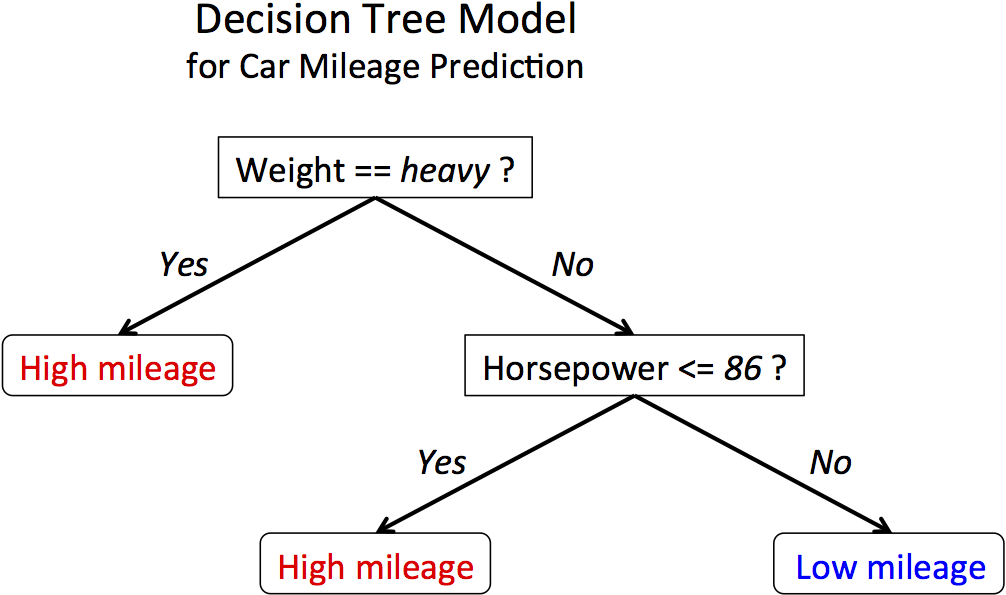
\includegraphics[width=0.6\linewidth]{pic/decision_trees.png}
  \caption{Decision Tree Example}
  \label{fig:dr_eg}
\end{figure}
\end{frame}

\begin{frame}{Gradient Boosting Trees}
Boosting is an ensemble technique in which the predictors are not made independently, but sequentially. This method tries to fit the new redictor to the residual errors made by the previous predictor. 
\begin{figure}
  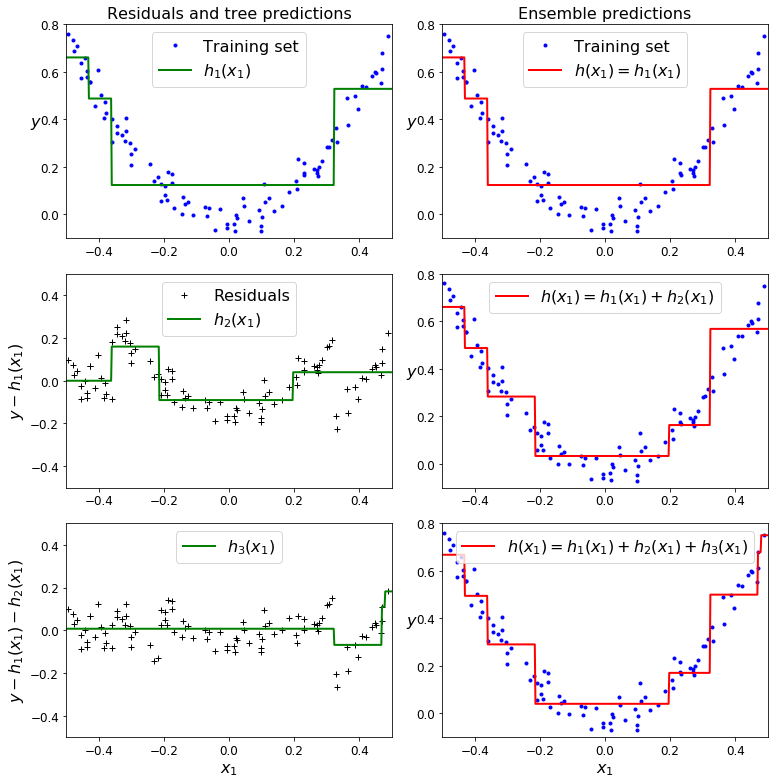
\includegraphics[width=0.45\linewidth]{pic/gradient_boosting.png}
  \caption{Gradient Boosting Tree Eaxmple}
  \label{fig:gbt_eg}
\end{figure}

\end{frame}



\begin{frame}
\frametitle{Models}
\begin{block}{Logistic Regression}
Easy to implement and very efficient to train.\\
Feature engineering plays an important roles. \\
Only produce linear decision boundary. \\
 Data needs to be well preprocessed. \\
\end{block}

\begin{block}{Decision Tree}
Less data cleaning is requires (NAN). \\
Data type is not a constraint. \\
Implicitly perform feature selections.\\
Slower and overfitting. 
\end{block}

\begin{block}{LightGBM}
Model is more powerful compared to decision tree.\\
Fast compared to gradient boosting tree.\\
\end{block}
\end{frame}

%------------------------------------------------

\begin{frame}{Pipeline}
\begin{itemize}
\item Preprocess train and test data. 
\item Data augmentation. 
\item Feature Selection using LightGBM
\item Logistic Regression, Decision Trees and LightGBM models. 
\item Bayesian optimization for LightGBM. 
\item Model Ensemble. 
\end{itemize}
\end{frame}

\begin{frame}{Feature Importance}
\begin{figure}
\centering
\begin{subfigure}{.5\textwidth}
  \centering
  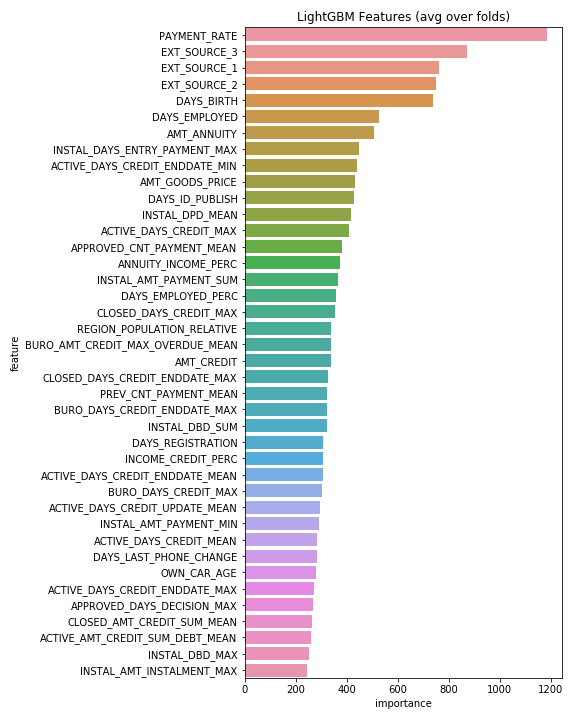
\includegraphics[width=.4\linewidth]{pic/lgbm_importances01.png}
  \caption{LightGBM Importances}
  \label{fig:sub1}
\end{subfigure}%
\begin{subfigure}{.5\textwidth}
  \centering
  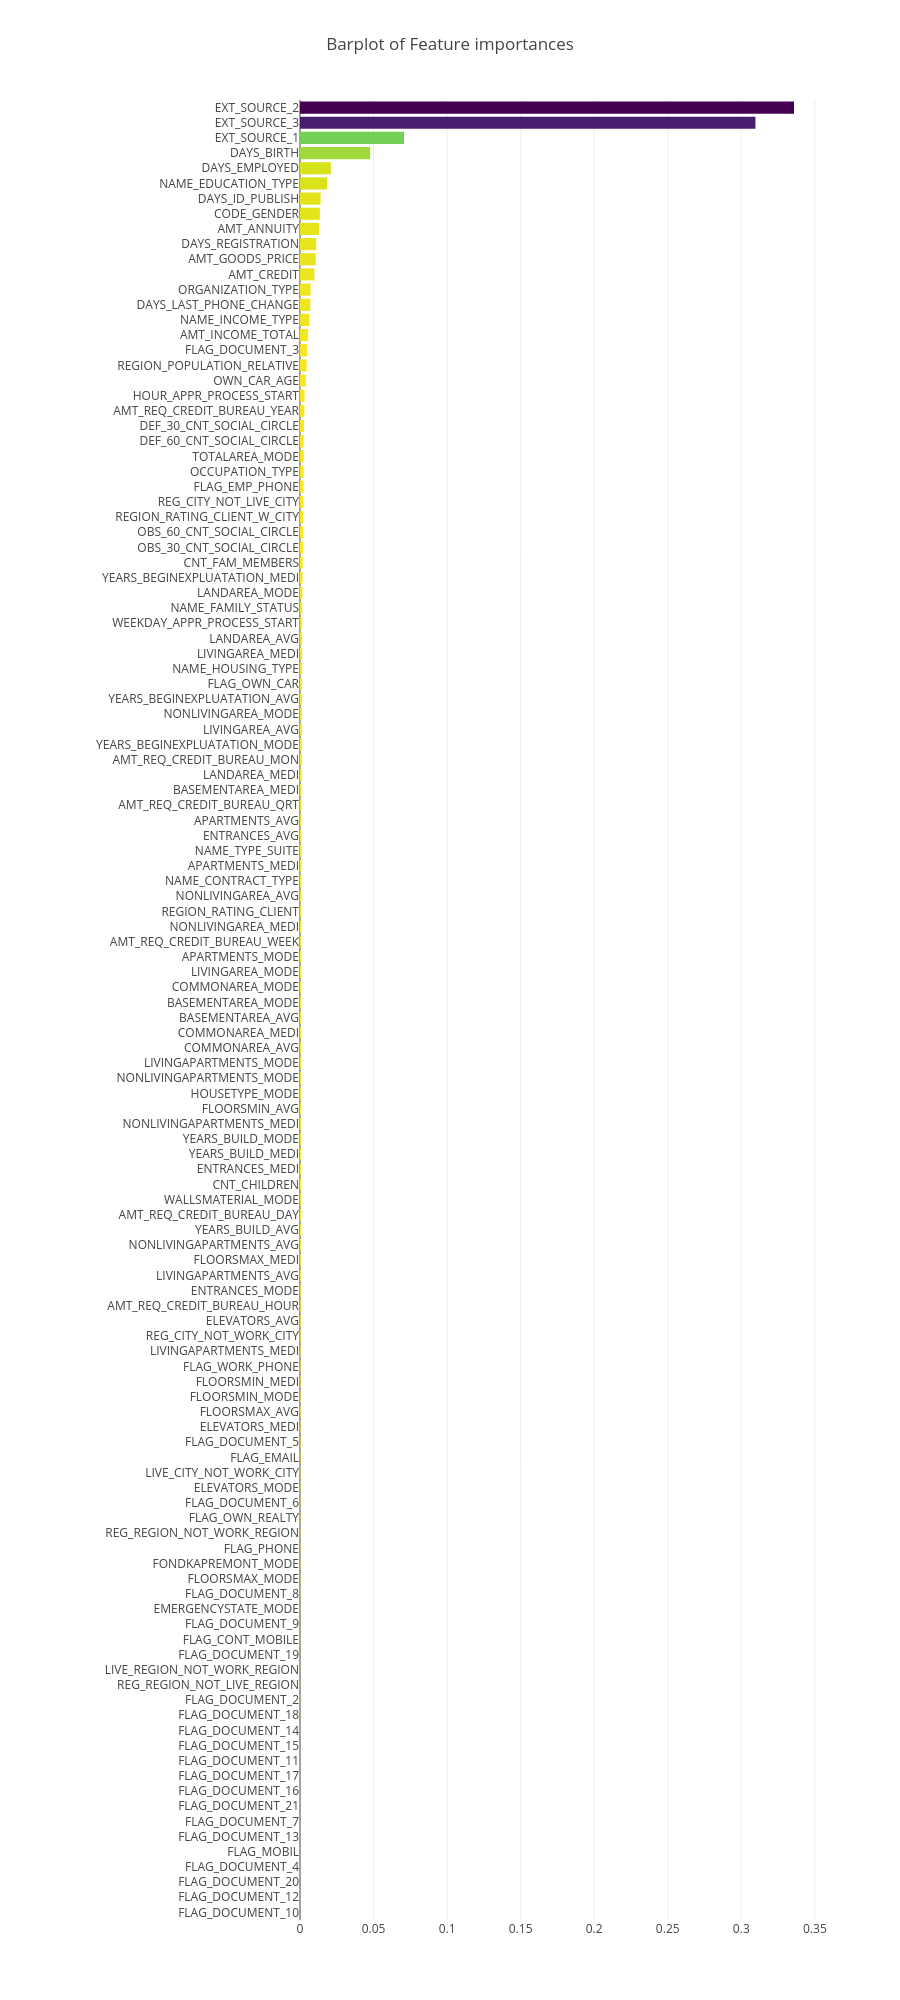
\includegraphics[width=.4\linewidth]{pic/dr_importances.png}
  \caption{Decision Tree Importances}
  \label{fig:sub2}
\end{subfigure}
\caption{Feature Importances}
\label{fig:feature_importances}
\end{figure}
\end{frame}

%------------------------------------------------
\section{Second Section}
%------------------------------------------------

\begin{frame}{Results: AUC Scores}
\begin{figure}
  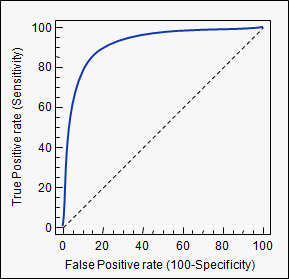
\includegraphics[width=0.4\linewidth]{pic/auc_scores.png}
  \label{fig:auc}
\end{figure}
\begin{table}
\begin{tabular}{l l l}
\toprule
\textbf{Logistic Regression} & \textbf{Decision Tree} & \textbf{LightGBM}\\
\midrule
0.671 & 0.678 & 0.787 \\
\bottomrule
\end{tabular}
\caption{AUC Scores}
\end{table}
\end{frame}

%------------------------------------------------

\begin{frame}{Improvements}
\begin{itemize}
\item Make more use of EDA. 
\item Use Neural Networks as one model. 
\item Ensemble various models.
\item Light feature selections. 
\end{itemize}

\end{frame}

%------------------------------------------------

\begin{frame}
\Huge{\centerline{Thank you!}}
\end{frame}

%----------------------------------------------------------------------------------------

\end{document} 